\chapter{Logik}
\section{Was ist Logik?}
\textit{''Septem artes liberalen''}, 7 freie Künste \\
Fächerkanon:
\begin{itemize}
	\item Trivium
	\begin{itemize}
		\item Grammatik
		\item Rhetorik
		\item Logik
	\end{itemize}
	\item Quadrivium
	\begin{itemize}
		\item Arithmetik
		\item Geometrie
		\item Musik
		\item Astronomie
	\end{itemize}
\end{itemize}
$\drsh$ ''trivial'' \\
''logos'': argumentierende, begründende Rede, vernünftiges Sprechen \\
Logik: Lehre des Begründens, Argumentierens, Schliessens \\
\begin{tabular}{lll}
	1918:	& Frege:	& $\frac{\text{schön}}{\text{Ästhetik}} = \frac{\text{gut}}{\text{Ethik}} = \frac{\text{wahr}}{\text{Logik}}$ \\
	1970:	& Patzig:	& Logik = Theorie der Aussagen, die aufgrund \textbf{ihrer Form} wahr sind. \\
	1985:	& Menne:	& Logik = Lehre von der \textbf{Folgerichtigkeit}
\end{tabular}
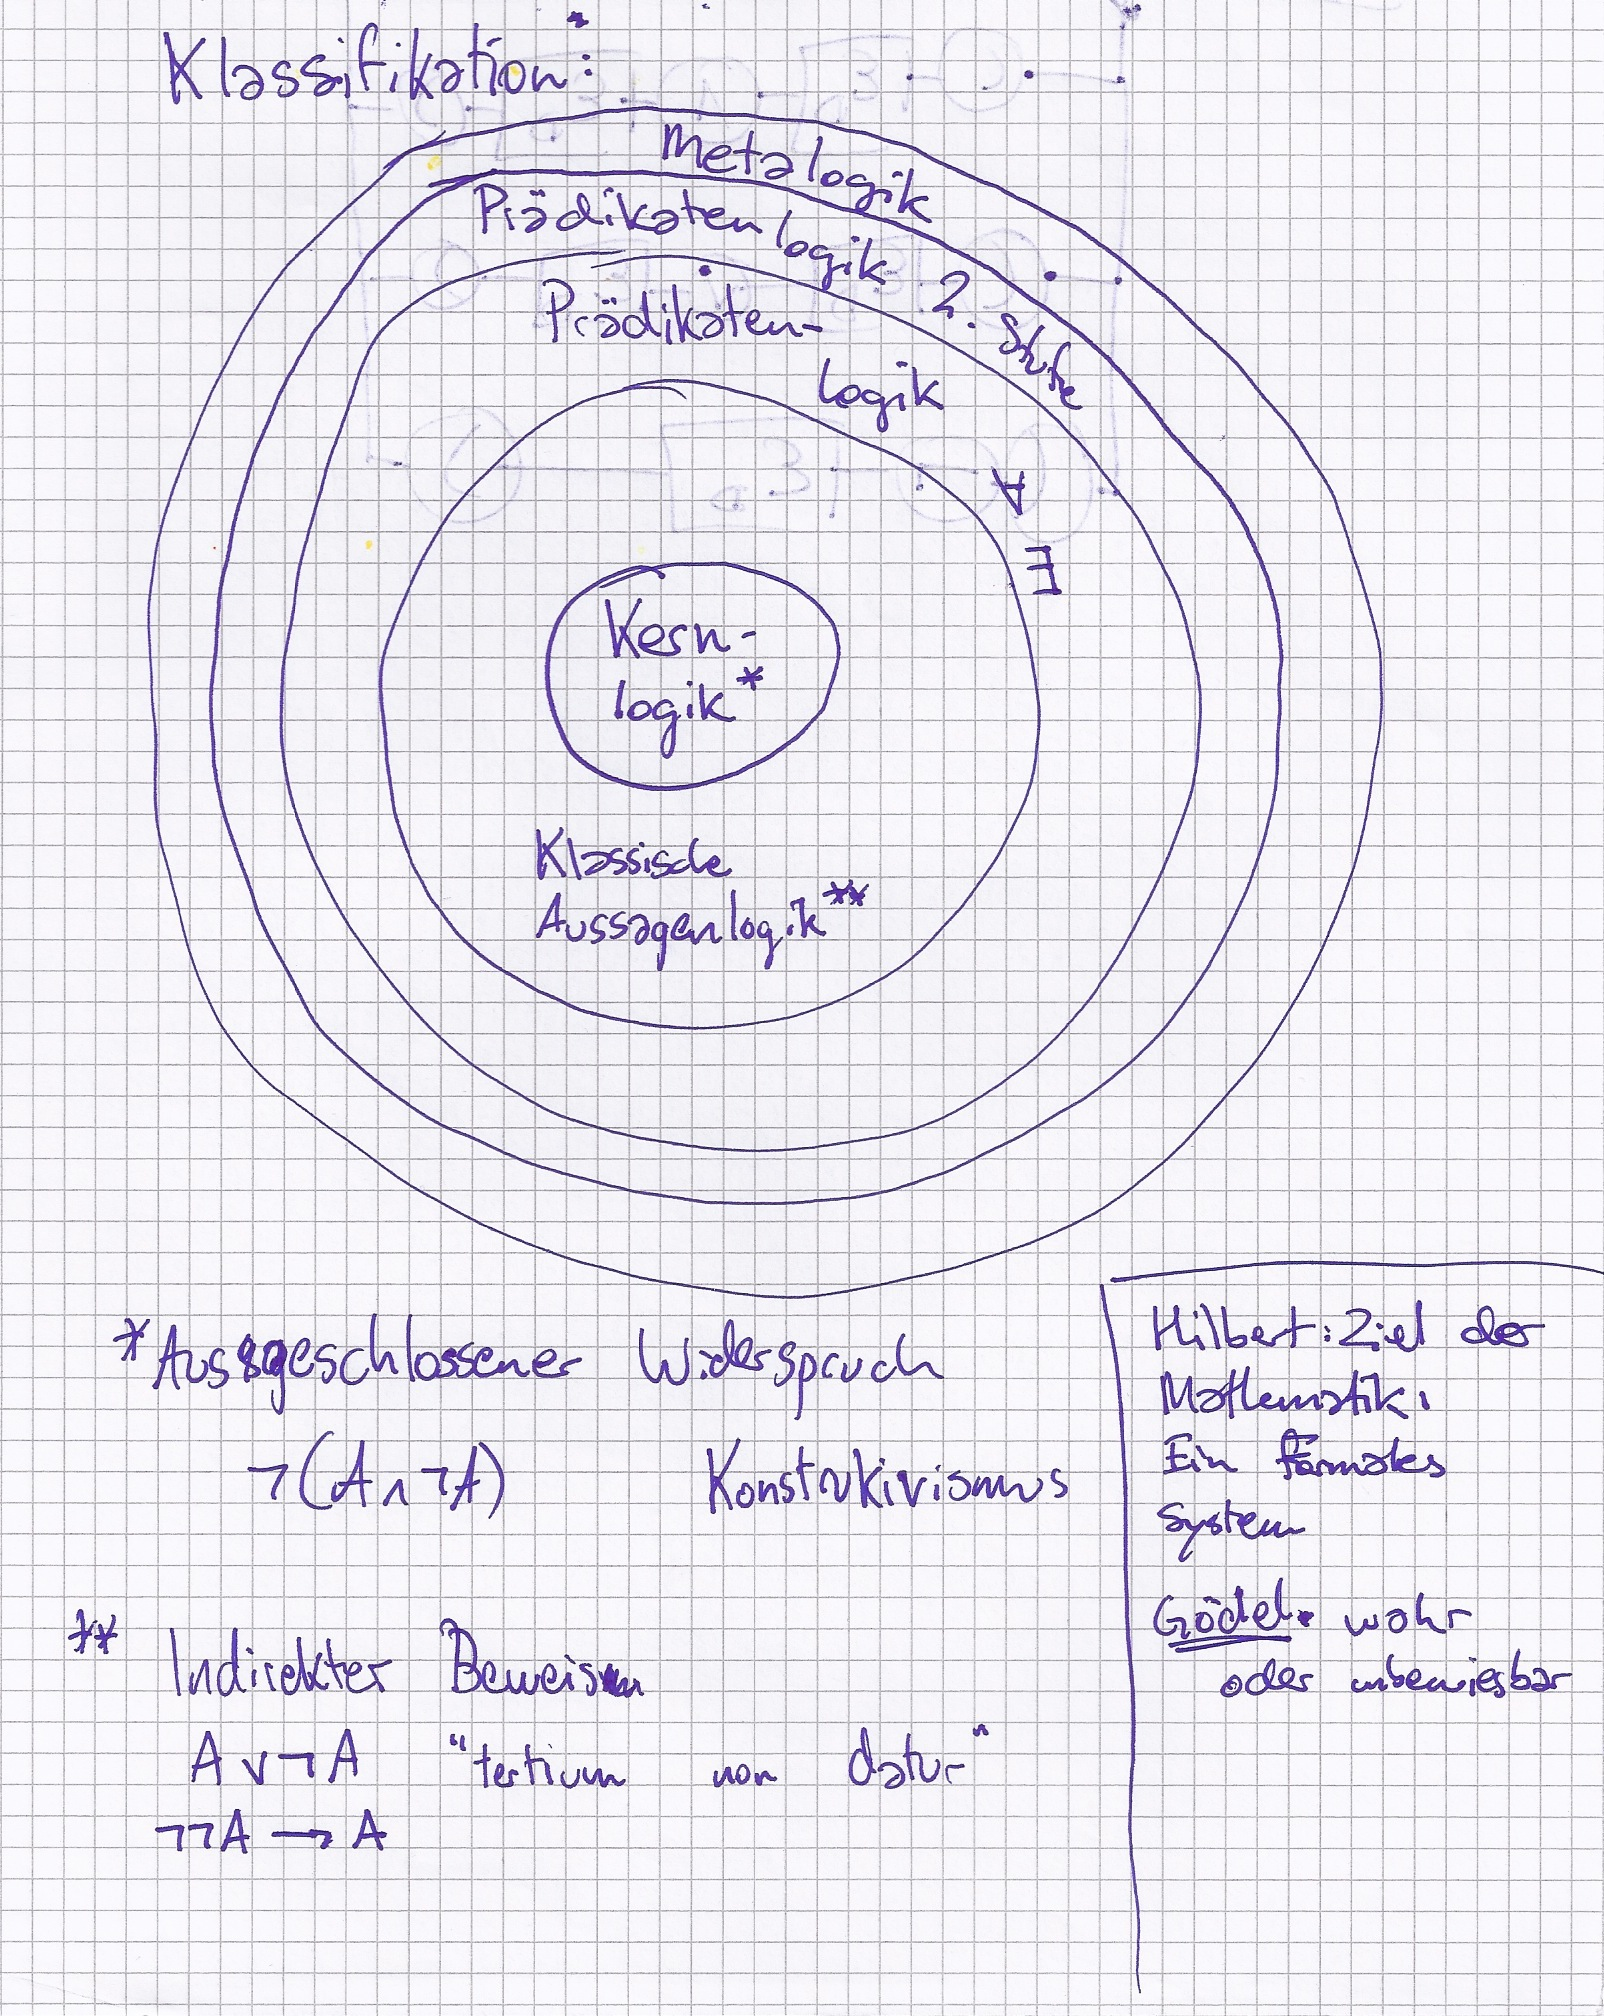
\includegraphics[width=\textwidth]{Bild6} \\
\begin{bsp*}
	Gibt es $r_1 , r_2 \notin \Q \text{ mit } {r_1}^{r_2} \in \Q$ ? Ja.
	\begin{gather*}
		\sqrt{2} \notin \Q \qquad
		\begin{bmatrix*}{l} \todo{Fix equation}
			%\sqrt{2} = \frac{p}{q} \rightarrow 2p^2 = q^2 \rightarrow p = 2p' \rightarrow 2p^2 = 4p'^2 \\
			\implies \text{Bruch nicht gekürzt.}
		\end{bmatrix*} \\
		\sqrt{2}^{\sqrt{2}} \in \Q \vee \sqrt{2}^{\sqrt{2}} \notin \Q \qquad \sqrt{2}^{{\sqrt{2}}^{\sqrt{2}}} = 2
	\end{gather*}
\end{bsp*}
